\documentclass{article}

\usepackage[english]{babel}

\usepackage[letterpaper,top=2.5cm,bottom=2.5cm,left=2.5cm,right=2.5cm,marginparwidth=1.75cm]{geometry}

\usepackage{amsmath}
\usepackage{graphicx}
\usepackage[colorlinks=true, allcolors=blue]{hyperref}
\usepackage{cancel, fancyhdr, textcomp, subfig}
\usepackage{bm}
\usepackage[export]{adjustbox}

\renewcommand{\thesubfigure}{}
\captionsetup[subfigure]{labelformat=simple, labelsep=colon}
\pagestyle{fancy}
\fancyhf{}
\rhead{Jacob Sigman}
\lhead{CE-341 Notes}
\cfoot{\thepage}
\renewcommand{\headrulewidth}{1.5pt}
\setlength{\headheight}{22.6pt}

\begin{document}
\section*{January 18th, 2023}
The first beam was an \textbf{``S'' Shape}. The top and bottom sections of the shape are called the \textbf{flange} and the middle section of the shape is called the \textbf{Web}. The shape has a \(16\,\frac{2}{3}\%\) slope, getting thicker as the flange approaches the web. The issue with this shape is when it was bolted the slope interfered with the top nut of any bolt you would put in, making it impossible to tighten. Due to this inefficiency the \textbf{``W'' Shape} was created, with longer flanges, a thin web, and no slope.
\begin{center}
    \vspace{3mm}
    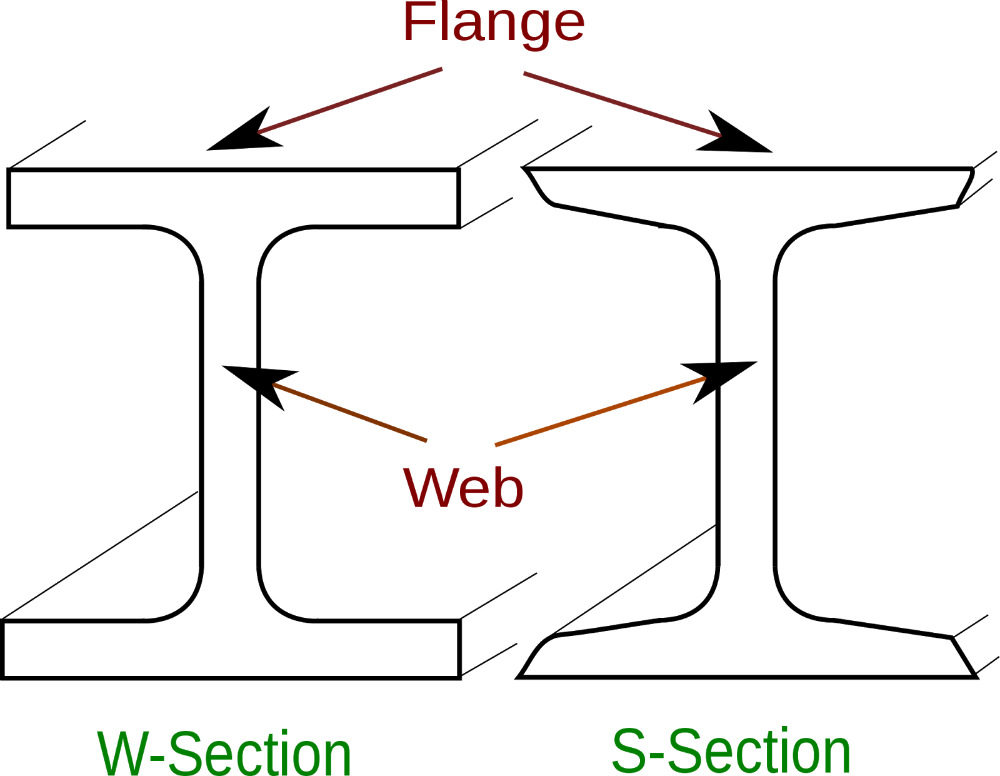
\includegraphics[scale=0.2]{fig1.jpg}
    \vspace{3mm}
    \\Figure 1: W and S Shapes
\end{center}
\noindent A steel shape has many values. \(\bm{t_w}\) is the thickness of the web, \(\bm{t_f}\) is the thickness of the flange, \(\bm{b_f}\) is the approximate length of the flange, and \(\bm{d}\) is the approximate depth. An example of a shape is W18x50, meaning that the shape is a W shape, with a \(\bm{d}\) measurement of approximately 18 feet, and a distributed weight of 15 pounds per foot.
\begin{center}
    \vspace{3mm}
    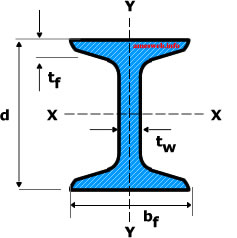
\includegraphics[scale=1]{fig2.jpg}
    \vspace{3mm}
    \\Figure 2: Measurements of a Steel S Shape
\end{center}
\newpage
\noindent \textbf{Steel} is composed of many chemicals. It's approximately 98\% iron, less than 1\% carbon, and about 1\% manganese, nickle, silicon, and sulfur. Another kind of steel is \textbf{``Mild Steel''}, intended for structural purposes, which contains about 0.15\% - 0.29\% carbon. The \textbf{Stress-Strain Curve} for steel determines how it fails and deforms. The slope of the stress strain curve is called the \textbf{Young's Modulus}, and is only applicable in the \textbf{Elastic Region}, where the idealized stress-strain curve has a positive slope. Farther along past failure is the point of \textbf{Ultimate Failure}. The approximate Young's Modulus of mild steel is 29,000 kips per square inch.
\begin{center}
    \vspace{3mm}
    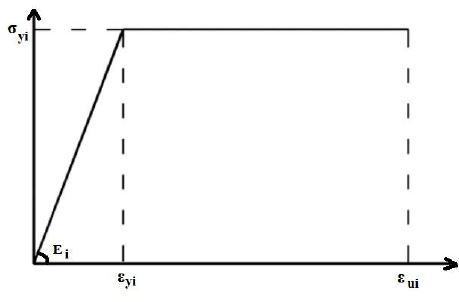
\includegraphics[scale=0.5]{fig3.png}
    \vspace{3mm}
    \\Figure 3: Idealized Stress-Strain Curve for Steel
\end{center}
\noindent Another type of section is an \textbf{``L'' Shape}, also called and \textbf{Angle}, typically used in connections. An example of an L shape is L5x3\textonehalf x\textonehalf, meaning the shape is 5 inches tall, 3\(\frac{1}{2}\) inches wide, and \(\frac{1}{2}\) inch thick. If there is a 2 preceding the measurement, it means the connection is a double-angle connection. Another type of section is a \textbf{``C'' Shape}, shown below. An example of a C shape is C10x15.3, which is 10 inches tall and 15 inches wide.
\begin{figure}[!ht]
    \centering
    \subfloat[Figure 4: L Shape]{
        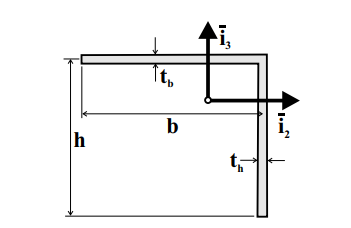
\includegraphics[width=0.4\linewidth]{fig4.png}
        }
    \subfloat[Figure 5: C Shape]{
        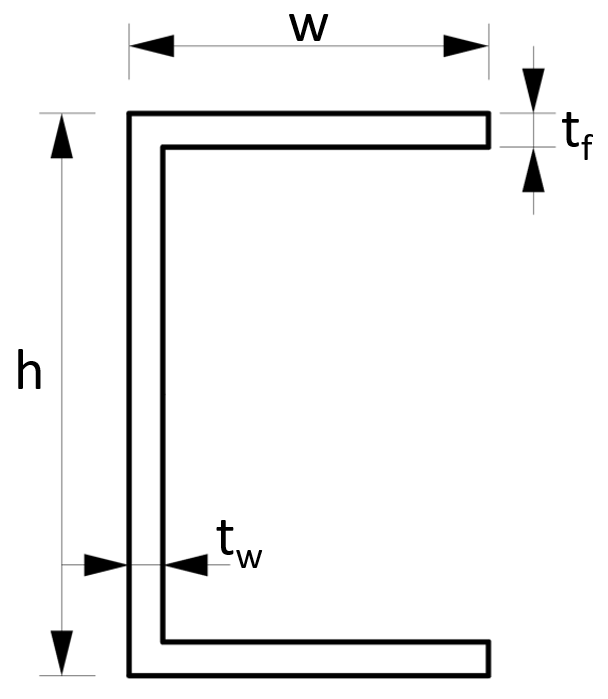
\includegraphics[scale=0.5]{fig5.png}
        }
\end{figure}
\\
\noindent There are two types of design. The first kind is ASD, or \textbf{Allowable Stress Design}, in existence since the 1880s. The second kind is LRFD, or \textbf{Load and Resistance Factor Design}, in existence since 1986. The following equation is used for LRFD.
\[\sum_i\,\gamma_i\, Q_i\leq \phi\, R_n\] 
\noindent Where \(\gamma_i\) is the load factor, \(Q_i\) is the load, \(\phi\) is the strength reduction factor, and \(R_n\) is the nominal strength. The following equation is used for ASD. 
\[\sum_i\, Q_i\leq\frac{R_n}{\Omega}\]
\noindent Where \(Q_i\) is the load, \(R_n\) is the nominal strength, and \(\Omega\) is the overall safety factor. 
\newpage
\noindent There are also various \textbf{Load Combinations} that you can use for ASD or LRFD. The full set of load combinations can be found in the textbook. Dead load is denoted by $D$, live load is denoted by $L$, roof live load is denoted by $L_r$, snow live load is denoted by $S$, earthquake live load is denoted by $E$, wind live load is denoted by $W$, and rain live load is denoted by $R$. Some examples for ASD are:
\begin{enumerate}
    \item $D$
    \item $D+L$
    \item $D+(L_r \text{ or } S \text{ or } R)$
    \item $D+0.75L+0.75\,(0.7E)$
\end{enumerate}
\noindent Some examples for LRFD are:
\begin{enumerate}
    \item $1.4D$ 
    \item $1.2D+1.6L+0.5\,(L_r \text{ or } S \text{ or } R)$
    \item $1.2D+1.0W+0.5L+0.5\,(L_r \text{ or } S \text{ or } R)$
    \item $1.2D+1.0E+0.5L+0.2S$
\end{enumerate}
\noindent ASD and LRFD also have a substantial relationship. As LRFD was introduced, it was calibrated to be similar to ASD. Upon it's introduction the calibration for LRFD was done for the case of $L=3D$. Which means that the $D+L$ load combination for ASD becomes $4D$ and the $1.2D+1.6L$ load combination for LRFD becomes $6D$. For ASD the capacity equation for the load combination is as follows:
\[\frac{R_n}{\Omega}=4D\] 
For LRFD the capacity equation for the load combination is as follows: 
\[\phi\, R_n=6D\]
From these two equations a relationship can be found between $\phi$ and $\Omega$. This relationship is used for every load combination. Starting with Chapter 3 only LRFD will be used in this course.
\[\Omega = \frac{1.5}{\phi}\]

\section*{January 25th, 2023}

This discussion entails the design of tension members, which is part 16 in the steel manual and chapter 3 in the textbook. 
\begin{enumerate} 
    \item Tension yielding on gross area. The goal is to avoid yielding since it increases the risk of rupture. This is a limit state.
    \item Tension rupture on effective net area. This is also a limit state.
    \item Block shear.
\end{enumerate} 

\begin{center}
    \vspace{3mm}
    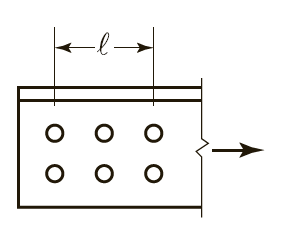
\includegraphics[scale=0.7]{fig6.png}
    \vspace{3mm}
    \\Figure 6: Steel Member
\end{center}
\newpage
\noindent Assume the thickness of the member to be $t$ and the height of the member to be $d$. The cross-sectional area \emph{without bolts} is as follows: 
\[A = d\times t\] 
The cross-sectional area \emph{with bolts} given that the diameter of each hole is $d_{h_\text{design}}$, is as follows: 
\[A_\text{net} = (d-2\times d_{h_\text{design}})\times t\] 
The first design is the \underline{standard} diameter for a hole: 
\[d_{h_\text{standard}}=d_b+x\] 
$x$ is 1/16" when $d_b$ is less than 1" and $x$ is 1/8" when $d_b$ is greater than or equal to 1". This can be found in table J3.3. The next step is the \underline{design} diameter for the hole. 
\[d_{h_\text{design}}=d_{h_\text{standard}}+1/16"\] 
This is to account for possible damage around the hole perimeter during fabrication.  The effective net area is as follows: 
\[A_e=U\times A_\text{net}\] 
Where $U$ is the \textbf{Shear Lag Factor} or eccentricity. More information on this can be found in Table D3.1. The \textbf{Interface Plane} is the plane where two members meet. The \textbf{Leg} of an angle is denoted by a double line on the front view. It is important to ensure that the connection length is in the same direction as the the ultimate tensile force. The equation used for a standard angle connecting to a plate is the equation from case 2 in table D3.1: 
\[U=1-\frac{\bar{x}}{L}\] 
Back to our initial discussion: 
\begin{enumerate}
    \item Tension Yielding: \(\phi\times R_n = 0.9\times F_y\times A\) 
    \item Tension Rupture: \(\phi\times R_n = 0.75\times F_u\times A_e\)
    \item Block Shear: There are two types of shear failure, the first being yielding and the second being rupture, however the only type of tensile failure is rupture. The equation is: 
    \begin{multline*} \phi\times R_n=0.75\times \text{Min}(0.6\,F_y\,L_V\,t+U_{bs}\,F_u\,(L_t-1.5\,d_{h_\text{design}})t,\\\, 0.6\,F_u\,(L_V-2.5\,d_{h_\text{design}})t+U_{bs}\,F_u\,(L_t-1.5\,d_{h_\text{design}})t)
    \end{multline*}
\end{enumerate}
$L_V$ is defined at the shear length, $U_{bs}$ is defined as the ultimate block shear, and $L_t$ is defined as the tensile length. Typically $U_{bs}$ is taken as 1. \textbf{Staggered Holes} is another complication that could arise in the design of tension members. These are holes that aren't necessarily lined up. If you don't want to change the thickness of the steel, staggering the holes is the solution. In order to determine if the staggered holes are placed properly according to edge distance, investigate all possible paths and the smallest strength will govern what needs to be designed for. Gage distances for angles can be found in table 1-7A. For diagonal paths, the net effective area is taken as follows: 
\[A_n=A+\sum\left[\left(\frac{s^2}{4g}\right)\times(t)\right]-\sum\left[ n_\text{holes}\times d_{n_{st}}\times t\right]\] 
Where $s$ is the stagger dimension and $g$ is the gage. For C-shapes, when the thickness of the flange differs substantially from the thickness of the web, ensure to follow the centerline and make the required adjustments by using the unweighted average of the two thicknesses.
\section*{February, 1st, 2023}
The next discussion is with regard to the design of compression members. The primary concern is the design of columns to ensure that they do not buckle under load. Below is an image showing column buckling: 
\begin{center}
    \vspace{3mm}
    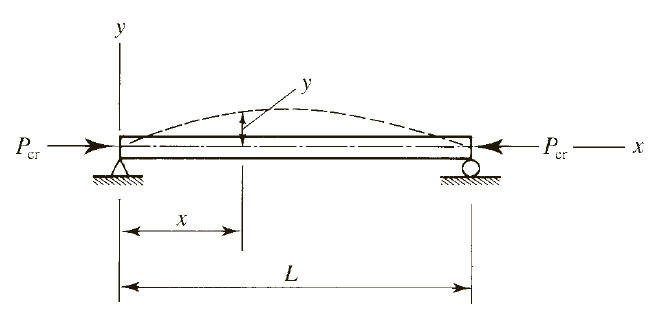
\includegraphics[scale=0.7]{fig7.png}
    \vspace{3mm}
    \\Figure 7: Column Buckling
\end{center}
Taking the sum of moments yields the following: 
\[\sum M_x=0\hspace{5mm} M-Py=0\hspace{5mm}M=Py\]
The next important piece of information is the equation of beam deflection, which is as follows: 
\[EI\frac{d^2y}{dx^2}=-M=-Py\hspace{5mm}EI\frac{d^2y}{dx^2}+Py=0\] 
Divide by EI, and let $\lambda^2=\frac{P}{EI}$: 
\[\frac{d^2y}{dx^2}+\lambda^2y=0\] 
This gives the differential equation form of deflection. Solving the equation involves taking a guess of $y=e^{\alpha x}$.
\[y'=\alpha e^{\alpha x}\hspace{5mm}y''=\alpha^2e^{\alpha x}\hspace{5mm}e^{\alpha x}(\alpha^2+\lambda^2)=0\] 
\[\alpha^2+\lambda^2=0\hspace{5mm}\alpha=\pm i\lambda\] 
\[y_1=e^{i\lambda x}\hspace{5mm}y_2=e^{-i\lambda x}\] 
Using Euler's Formula and the principle of superposition, the following is obtained: 
\[y=c_1(\cos\lambda x+i\sin\lambda x)+c_2(\cos\lambda x - i\sin\lambda x)\] 
Since the solution is real, $c_1$ and $c_2$ have to be complex conjugates, giving that $c_1=a+bi$ and $c_2=a-bi$. This ensures that in both addition and subtraction of the two constants, the solution is real. Letting $c_1+c_2=A$ and $i(c_1-c_2)=B$. This substitution yields the following: 
\[y=A\cos \lambda x+B\sin \lambda x\] 
Boundary conditions are used to find $A$ and $B$. We know that $y(0)=0 and y(L)=0$. These two conditions are sufficient to determine $A$ and $B$. The first boundary condition yields 0 for $A$. However, the second boundary condition cannot yield 0 for $B$. Therefore, $\lambda L$ must be a multiple of $\pi$. 
\[\lambda L = n\pi \hspace{3mm}n\neq0\]
The objective is to find the lowest possible eigenvalue for design ($n=1$). 
\[\lambda L = \pi\hspace{5mm}P_{cr}=\frac{\pi^2EI}{L^2}\] 
Another useful parameter is the \textbf{radius of gyration}, or $r$. 
\[r=\sqrt{\frac{I}{A}}\hspace{5mm}P_{cr}=\frac{\pi^2r^2AE}{L^2}\]
The most meaningful formula is the critical stress $F_{cr}$. 
\[F_{cr}=\frac{P_cr}{A}=\frac{\pi^2E}{\left(\frac{L}{r}\right)^2}\] 
Where $\frac{L}{r}$ is defined as the \textbf{slenderness ratio}. The objective is to not go above the yield strength. As a hot member cools, components of the member with different thicknesses won't have an even cooling rate. This leaves a \textbf{residual thermal stress}. There are many different $k$ factors for column buckling. For a column pinned at both ends, $k=1$. For a column fixed at both ends, $k=0.5$. A column pinned at one end at fixed at another has a $k$ of $0.7$. A column that is fixed at one end and free at another end has $k=2$.\\
With regard to stiffness, equations for $\tau$ can be found in section C3 and for $G$ in section CA-7. For now, we assume that members have no slender elements, so section E-3 would be the most relevant.
\end{document}